%-----------------------------------------------------------------------------------------------------------------------------------------------%
%	The MIT License (MIT)
%
%	Copyright (c) 2019 Jan Küster
%
%	Permission is hereby granted, free of charge, to any person obtaining a copy
%	of this software and associated documentation files (the "Software"), to deal
%	in the Software without restriction, including without limitation the rights
%	to use, copy, modify, merge, publish, distribute, sublicense, and/or sell
%	copies of the Software, and to permit persons to whom the Software is
%	furnished to do so, subject to the following conditions:
%	
%	THE SOFTWARE IS PROVIDED "AS IS", WITHOUT WARRANTY OF ANY KIND, EXPRESS OR
%	IMPLIED, INCLUDING BUT NOT LIMITED TO THE WARRANTIES OF MERCHANTABILITY,
%	FITNESS FOR A PARTICULAR PURPOSE AND NONINFRINGEMENT. IN NO EVENT SHALL THE
%	AUTHORS OR COPYRIGHT HOLDERS BE LIABLE FOR ANY CLAIM, DAMAGES OR OTHER
%	LIABILITY, WHETHER IN AN ACTION OF CONTRACT, TORT OR OTHERWISE, ARISING FROM,
%	OUT OF OR IN CONNECTION WITH THE SOFTWARE OR THE USE OR OTHER DEALINGS IN
%	THE SOFTWARE.
%	
%
%-----------------------------------------------------------------------------------------------------------------------------------------------%


%============================================================================%
%
%	DOCUMENT DEFINITION
%
%============================================================================%

%we use article class because we want to fully customize the page and don't use a cv template
\documentclass[10pt,A4]{article}	


%----------------------------------------------------------------------------------------
%	ENCODING
%----------------------------------------------------------------------------------------

% we use utf8 since we want to build from any machine
\usepackage[utf8]{inputenc}		

%----------------------------------------------------------------------------------------
%	LOGIC
%----------------------------------------------------------------------------------------

% provides \isempty test
\usepackage{xstring, xifthen}

%----------------------------------------------------------------------------------------
%	FONT BASICS
%----------------------------------------------------------------------------------------

% some tex-live fonts - choose your own

%\usepackage[defaultsans]{droidsans}
%\usepackage[default]{comfortaa}
%\usepackage{cmbright}
\usepackage[default]{raleway}
\usepackage{fontawesome}
%\usepackage{fetamont}
%\usepackage[default]{gillius}
%\usepackage[light,math]{iwona}
%\usepackage[thin]{roboto} 

% set font default
\renewcommand*\familydefault{\sfdefault} 	
\usepackage[T1]{fontenc}

% more font size definitions
\usepackage{moresize}

%----------------------------------------------------------------------------------------
%	FONT AWESOME ICONS
%---------------------------------------------------------------------------------------- 

% include the fontawesome icon set
\usepackage{fontawesome}

% use to vertically center content
% credits to: http://tex.stackexchange.com/questions/7219/how-to-vertically-center-two-images-next-to-each-other
\newcommand{\vcenteredinclude}[1]{\begingroup
\setbox0=\hbox{\includegraphics{#1}}%
\parbox{\wd0}{\box0}\endgroup}

% use to vertically center content
% credits to: http://tex.stackexchange.com/questions/7219/how-to-vertically-center-two-images-next-to-each-other
\newcommand*{\vcenteredhbox}[1]{\begingroup
\setbox0=\hbox{#1}\parbox{\wd0}{\box0}\endgroup}

% icon shortcut
\newcommand{\icon}[3] { 							
	\makebox(#2, #2){\textcolor{maincol}{\csname fa#1\endcsname}}
}	

% icon with text shortcut
\newcommand{\icontext}[4]{ 						
	\vcenteredhbox{\icon{#1}{#2}{#3}}  \hspace{2pt}  \parbox{0.9\mpwidth}{\textcolor{#4}{#3}}
}

% icon with website url
\newcommand{\iconhref}[5]{ 						
    \vcenteredhbox{\icon{#1}{#2}{#5}}  \hspace{2pt} \href{#4}{\textcolor{#5}{#3}}
}

% icon with email link
\newcommand{\iconemail}[5]{ 						
    \vcenteredhbox{\icon{#1}{#2}{#5}}  \hspace{2pt} \href{mailto:#4}{\textcolor{#5}{#3}}
}

%----------------------------------------------------------------------------------------
%	PAGE LAYOUT  DEFINITIONS
%----------------------------------------------------------------------------------------

% page outer frames (debug-only)
% \usepackage{showframe}		

% we use paracol to display breakable two columns
\usepackage{paracol}

% define page styles using geometry
\usepackage[a4paper]{geometry}

% remove all possible margins
\geometry{top=1cm, bottom=1cm, left=1cm, right=1cm}

\usepackage{fancyhdr}
\pagestyle{empty}

% space between header and content
\setlength{\headheight}{0pt}

% indentation is zero
\setlength{\parindent}{0mm}

%----------------------------------------------------------------------------------------
%	TABLE /ARRAY DEFINITIONS
%---------------------------------------------------------------------------------------- 

% extended aligning of tabular cells
\usepackage{array}

% custom column right-align with fixed width
% use like p{size} but via x{size}
\newcolumntype{x}[1]{%
>{\raggedleft\hspace{0pt}}p{#1}}%


%----------------------------------------------------------------------------------------
%	GRAPHICS DEFINITIONS
%---------------------------------------------------------------------------------------- 

%for header image
\usepackage{graphicx}

% use this for floating figures
% \usepackage{wrapfig}
% \usepackage{float}
% \floatstyle{boxed} 
% \restylefloat{figure}

%for drawing graphics		
\usepackage{tikz}				
\usetikzlibrary{shapes, backgrounds,mindmap, trees}

%----------------------------------------------------------------------------------------
%	Color DEFINITIONS
%---------------------------------------------------------------------------------------- 
\usepackage{transparent}
\usepackage{color}

% primary color
\definecolor{maincol}{RGB}{ 225, 0, 0 }

% accent color, secondary
\definecolor{accentcol}{RGB}{ 250, 150, 10 }

% dark color
\definecolor{darkcol}{RGB}{ 70, 70, 70 }

% light color
\definecolor{lightcol}{RGB}{245,245,245}


% Package for links, must be the last package used
\usepackage[hidelinks]{hyperref}

% returns minipage width minus two times \fboxsep
% to keep padding included in width calculations
% can also be used for other boxes / environments
\newcommand{\mpwidth}{\linewidth-\fboxsep-\fboxsep}
	

%============================================================================%
%
%	CV COMMANDS
%
%============================================================================%

%----------------------------------------------------------------------------------------
%	 EXT Link
%----------------------------------------------------------------------------------------

\newcommand{\extLink}[2]{
	\textcolor{maincol}{\href{#1}{#2}}
}

\newcommand{\extLinkIcon}[2]{
	\textcolor{maincol}{\href{#1}{#2 \,\scriptsize{\faExternalLink} }}
}
%----------------------------------------------------------------------------------------
%	 CV LIST
%----------------------------------------------------------------------------------------

% renders a standard latex list but abstracts away the environment definition (begin/end)
\newcommand{\cvlist}[1] {
	\begin{itemize}{#1}\end{itemize}
}

%----------------------------------------------------------------------------------------
%	 CV TEXT
%----------------------------------------------------------------------------------------

% base class to wrap any text based stuff here. Renders like a paragraph.
% Allows complex commands to be passed, too.
% param 1: *any
\newcommand{\cvtext}[1] {
	\begin{tabular*}{1\mpwidth}{p{0.98\mpwidth}}
		\parbox{1\mpwidth}{#1}
	\end{tabular*}
}

%----------------------------------------------------------------------------------------
%	CV SECTION
%----------------------------------------------------------------------------------------

% Renders a a CV section headline with a nice underline in main color.
% param 1: section title
\newcommand{\cvsection}[1] {
	\vspace{14pt}
	\cvtext{
		\textbf{\LARGE{\textcolor{darkcol}{\uppercase{#1}}}}\\[-4pt]
		\textcolor{maincol}{ \rule{0.1\textwidth}{2pt} } \\
	}
}

%----------------------------------------------------------------------------------------
%	META SKILL
%----------------------------------------------------------------------------------------

% Renders a progress-bar to indicate a certain skill in percent.
% param 1: name of the skill / tech / etc.
% param 2: level (for example in years)
% param 3: percent, values range from 0 to 1
\newcommand{\cvskill}[3] {
	\begin{tabular*}{1\mpwidth}{p{0.72\mpwidth}  r}
 		\textcolor{black}{\textbf{#1}} & \textcolor{maincol}{#2}\\
	\end{tabular*}%
	
	\hspace{4pt}
	\begin{tikzpicture}[scale=1,rounded corners=2pt,very thin]
		\fill [lightcol] (0,0) rectangle (1\mpwidth, 0.15);
		\fill [maincol] (0,0) rectangle (#3\mpwidth, 0.15);
  	\end{tikzpicture}%
}


%----------------------------------------------------------------------------------------
%	 CV EVENT
%----------------------------------------------------------------------------------------

% Renders a table and a paragraph (cvtext) wrapped in a parbox (to ensure minimum content
% is glued together when a pagebreak appears).
% Additional Information can be passed in text or list form (or other environments).
% the work you did
% param 1: time-frame i.e. Sep 14 - Jan 15 etc.
% param 2:	 event name (job position etc.)
% param 3: Customer, Employer, Industry
% param 4: Short description
% param 5: work done (optional)
% param 6: technologies include (optional)
% param 7: achievements (optional)
\newcommand{\cvevent}[8] {
	
	% we wrap this part in a parbox, so title and description are not separated on a pagebreak
	% if you need more control on page breaks, remove the parbox
	\parbox{\mpwidth}{
		\begin{tabular*}{1\mpwidth}{p{0.72\mpwidth}  r}
	 		\textcolor{black}{\textbf{#2}} & \colorbox{maincol}{\makebox[0.28\mpwidth]{\textcolor{white}{#1}}} \\
			\textcolor{maincol}{\textbf{#3}} \ifthenelse{\isempty{#4}}{}{\textcolor{maincol}{\emph{- #4}}}  & \\
		\end{tabular*}\\[8pt]
	
		\ifthenelse{\isempty{#5}}{}{
			\cvtext{#5}\\
		}
	}

	\ifthenelse{\isempty{#6}}{}{
		\vspace{4pt}
		{#6}
	}

	\ifthenelse{\isempty{#7}}{}{
		\vspace{4pt}
		\cvtext{\textbf{Technologies include:}}\\
		{#7}
	}

	\ifthenelse{\isempty{#8}}{}{
		\vspace{4pt}
		\cvtext{\textbf{Achievements include:}}\\
		{#8}
	}
	\vspace{14pt}
}

%----------------------------------------------------------------------------------------
%	 CV META EVENT
%----------------------------------------------------------------------------------------

% Renders a CV event on the sidebar
% param 1: title
% param 2: subtitle (optional)
% param 3: customer, employer, etc,. (optional)
\newcommand{\cvmetaevent}[4] {
	\textcolor{maincol} {\cvtext{\textbf{\begin{flushleft}#1\end{flushleft}}}}
	\ifthenelse{\isempty{#2}}{}{
	\textcolor{darkcol} {\cvtext{\textbf{#2}} }
	}
	\ifthenelse{\isempty{#3}}{}{
		\cvtext{{ \textcolor{darkcol} {#3} }}\\
	}
}

%============================================================================%
%
%
%
%	DOCUMENT CONTENT
%
%
%
%============================================================================%
\begin{document}
\columnratio{0.77}
\setlength{\columnsep}{2.2em}
\setlength{\columnseprule}{4pt}
\colseprulecolor{lightcol}
\begin{paracol}{2}
\begin{leftcolumn}
%---------------------------------------------------------------------------------------
%	TITLE  HEADER
%----------------------------------------------------------------------------------------
\begin{minipage}[c][3.5cm][c]{1\mpwidth}
	\begin {center}
		\HUGE{ \textbf{ \textcolor{black}{ \uppercase{ Paolo Tagliani } } } } \\[-24pt]
		\textcolor{black}{ \rule{0.1\textwidth}{1.25pt} } \\[4pt]
		\large{ \textcolor{black} {Senior Freelance Software Engineer} }
	\end {center}
\end{minipage} \\[14pt]

%---------------------------------------------------------------------------------------
%	PROFILE
%----------------------------------------------------------------------------------------
\cvsection{PROFILO}

\cvtext{ Ingegnere del software con una solida preparazione tecnica e pratica, contribuisce e sostiene varie librerie OpenSource.\\

Oltre dieci anni di esperienza nella progettazione ed implementazione di applicazioni mobile e web. Lavoro remoto dal 2015.\\

Orientato alle esigenze del cliente e con una metodologia di lavoro strutturata, focalizzata sulla qualità del codice e sulla manutenzione. Ottima capacità di lavoro in team, sia in grandi aziende che in team di piccola-media dimensione.
}

%---------------------------------------------------------------------------------------
%	WORK EXPERIENCE
%----------------------------------------------------------------------------------------
\cvsection{ESPERIENZE LAVORATIVE}

\cvevent
	{Gen 2021 - Giu 2022}
	{Linux/FullStack Developer - iOS Developer}
	{\extLinkIcon{https://www.masterchart.it/}{Masterchart}}
	{Hybrid Remote}
	{Design ed implementazione di un sistema di controllo degli accessi per il settore bancario, composto da differenti applicativi frontend e da una distribuzione linux creata ad-hoc per kiosk e soluzioni Digital Signage.}
	{\cvlist{
		\item Piattaforma Prenotabanca (\extLink{https://www.masterchart.it/prenota-banca.html}{link})
	}}
	{}
	{}

\cvevent
	{Mar 2021 - Giu 2021}
	{Linux/FullStack developer}
	{\extLinkIcon{https://41north.dev/}{41 North}}
	{Full Remote}
	{Creazione di una distribuzione linux custom (basata su RaspiOS) pensata per l'installazione in soluzioni bartop per retro-gaming. Il sistema include anche un applicativo backend per la distribuzione di ROM legali. Maggiori dettagli a \extLink{https://talentec.es}{questo link}.}
	{}
	{}
	{}

\cvevent
	{Gen 2020 - Dic 2020}
	{Mobile and Full Stack Software Engineer}
	{\extLinkIcon{https://codermine.com/}{Codermine}}
	{Hybrid Remote}
	{Design ed implementazione di soluzioni mobile e web per clienti terzi. Leadership del team web, con attività che includono: menroting di sviluppatori junior, introduzione di pratiche DevOps, miglioramento del ciclo di sviluppo e introduzione di CI/CD e test automatici.\\
	 Qui un esempio di alcuni dei prodotti sviluppati:}
	{\cvlist{
		\item App di configurazione per un sistema di allarmi radar (\extLink{https://apps.apple.com/it/app/inxpect-security/id1334620177}{link})
		\item Piattaforma di trading di credito (frontend e backend) (\extLink{https://cashme.it/}{link})
		\item Piattaforma di predizione KPI basata su intelligenza artificiale (\extLink{https://vedrai.com/en/}{link})
	}}
	{}
	{}

\cvevent
	{Ago 2019 - Dic 2019}
	{Mobile / FullStack Software Engineer}
	{\extLinkIcon{https://www.palmabit.com/en}{Palmabit}}
	{Hybrid Remote}
	{Consulente full stack.}
	{\cvlist{
		\item Sistema di consegne basato su circular economy (\extLink{https://www.siwego.com/}{Link})
		\item Applicativo di chat basato su Bluetooth (\extLink{https://apps.apple.com/it/app/forcatch/id1372788996}{link})
	}}
	{}
	{}

\cvevent
	{Lug 2015 - Lug 2019}
	{Mobile / Full Stack Software Engineer}
	{\extLinkIcon{https://mobilejazz.com/}{MobileJazz}}
	{Full Remote}
	{Consulenza tecnica e manageriale per clienti basati in Europa e Stati Uniti. Nel percorso aziendale sono stati ricoperti i ruoli di sviluppatore iOS nel team mobile, in seguito sviluppatore team backend utilizzando tecnologie basate su Node.js ed infine sviluppo frontend nel team web. Responsabile per il DevOps, l'automazione e la creazione di sistemi di build automatica nei vari team. \\
	Alcuni degli esempi più rilevanti dei prodotti creati: }
	{\cvlist{
		\item Sistema di controllo delle luci IoT(\extLink{https://www.simonelectric.com/intl/control-systems/scena}{link}, \extLink{https://mobilejazz.com/blog/how-we-made-remote-development-work-with-physical-devices/}{blog post}) 
		\item Piattaforma di monitoraggio del rumore in real-time (\extLink{http://emmadb.com/}{link})
		\item Piattaforma per la riabilitazione post-operatoria (\extLink{https://peerwell.co/}{link})
		\item App per il controllo di un device TENS (\extLink{https://hollywog.com/products/witouch}{link})
		\item Applicazione di social networking per incontri (\extLink{https://apps.apple.com/us/app/koko-dating-flirt-chat-app/id855200334}{link}) 	}}
	{}
	{}

\cvevent
	{Mag 2013 - Giu 2015}
	{iOS Developer}
	{TilTap}
	{}
	{Sviluppatore iOS in un team dedicato allo sviluppo di MVP all'interno di un incubatore di startup. Creazione di prodotti per startup in fase di definizione prodotto. }
	{}
	{}
	{}

%---------------------------------------------------------------------------------------
%	SKILLS
%----------------------------------------------------------------------------------------
\cvsection{Competenze}

\begin{tabular*}{1\mpwidth}{p{1\mpwidth}  r}
	\textbf{Linguaggi di programmazione}\\
	\textcolor{maincol}{\textit{Esperto}}: Typescript, Swift, Objective-C/C++\\
	\textcolor{maincol}{\textit{Buona conoscenza}}: C, C++, Javascript, Python\\
	\textcolor{maincol}{\textit{Familiarità}}: Go, Ruby \\ 
	\\
	\textbf{DevOps}: GitHub Actions, Gitlab CI/CD Pipelines, Travis CI \\
	\\
	\textbf{Frameworks}: Cocoa, Cocoa Touch e framework iOS, NodeJS, NestJS, ExpressJS, Angular \\
	\\
	\textbf{DB}: MySQL, PostgreSQL, SQLite, MongoDB, Elastic Search, TimeScaleDB \\
	\\
	\textbf{Conainers}: Docker, Docker Compose, Kubernetes \\
	\\
	\textbf{Altre competenze}: Amministrazione Linux, AWS (S3, lambda, IoT, ECS), gestione di server cloud (Digital Ocean, Linode)
\end{tabular*}\\[8pt] 

%---------------------------------------------------------------------------------------
%	Projects
%----------------------------------------------------------------------------------------
\cvsection{Progetti personali e certificazioni}
\cvlist{
	\item \textbf{Brevetto US} Hazard Recognition (\extLinkIcon{https://patents.google.com/patent/US11093747B2/en?oq=US11093747B2
	}{Patent US11093747B2})
	\item Fondatore di \extLinkIcon{http://pragmamark.org/}{PragmaMark}: la prima conferenza italiana su iOS/macOSX
	\item Mentor presso \extLinkIcon{http://www.coderdojobrescia.it/}{CoderDojo Brescia}
}


% hotfixes to create fake-space to ensure the whole height is used
\mbox{}
\vfill
\mbox{}
\vfill
\mbox{}
\vfill
\mbox{}
\end{leftcolumn}
\begin{rightcolumn}
%---------------------------------------------------------------------------------------
%	META IMAGE
%----------------------------------------------------------------------------------------
\vfill \vspace*{110pt}
% 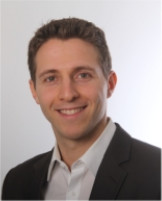
\includegraphics[width=\linewidth]{untitled.jpg}	%trimming relative to image size

%---------------------------------------------------------------------------------------
%	META CONTACT
%----------------------------------------------------------------------------------------
\cvsection{CONTATTI}
	
\icontext{MapMarker}{12}{Via Tormini 74/O, Gavardo (BS), Italy}{black}\\[6pt]
\icontext{MobilePhone}{12}{+39 329 2783809}{black}\\[6pt]
\iconemail{Envelope}{12}{pablosproject@gmail.com}{pablosproject@gmail.com}{black}\\[6pt]
\iconhref{Globe}{12}{pablosproject.com}{https://www.pablosproject.com}{black}\\[6pt]
\iconhref{Github}{12}{github.com/pablosproject}{https://github.com/pablosproject}{black}\\[6pt]
\iconhref{Linkedin}{12}{linkedin.com/in/paolo-tagliani}{https://www.linkedin.com/in/paolo-tagliani-51248117}{black}\\[6pt]

%---------------------------------------------------------------------------------------
%	EDUCATION
%----------------------------------------------------------------------------------------
\cvsection{EDUCAZIONE}

\cvmetaevent
{2010 - 2013}
{Laurea Magistrale in Ingegneria \mbox{Informatica}\\}
{Università degli studi di Brescia}
{}
\cvmetaevent
{2011 - 2012}
{Studente in visita, programma Erasmus\\}
{LaSalle Barcelona, Ramon Llull University}
{}
\cvmetaevent
{2006 - 2012}
{Laurea in Ingegneria dell'Informazione\\}
{Università degli studi di Brescia}
{}

%---------------------------------------------------------------------------------------
%	LANGUAGES
%----------------------------------------------------------------------------------------
\cvsection{LINGUE}
\cvlist{
	\item Italiano (lingua madre)
	\item Inglese
	\item Spagnolo
	\item Catalano
}

\vfill

\end{rightcolumn}
\end{paracol}
\end{document}

